
%%%%%%%%%%%%%%%%%%%%%%%%%%%%%%%%%%%%%%%%%%%%%%%%%%%%%%%%%%%%%%%%%%%%%%%%%%%%%%
%  ************************** AVISO IMPORTANTE **************************    %
%                                                                            %
% Éste es un documento de ayuda para los autores que deseen enviar           %
% trabajos para su consideración en el Boletín de la Asociación Argentina    %
% de Astronomía.                                                             %
%                                                                            %
% Los comentarios en este archivo contienen instrucciones sobre el formato   %
% obligatorio del mismo, que complementan los instructivos web y PDF.        %
% Por favor léalos.                                                          %
%                                                                            %
%  -No borre los comentarios en este archivo.                                %
%  -No puede usarse \newcommand o definiciones personalizadas.               %
%  -SiGMa no acepta artículos con errores de compilación. Antes de enviarlo  %
%   asegúrese que los cuatro pasos de compilación (pdflatex/bibtex/pdflatex/ %
%   pdflatex) no arrojan errores en su terminal. Esta es la causa más        %
%   frecuente de errores de envío. Los mensajes de "warning" en cambio son   %
%   en principio ignorados por SiGMa.                                        %
%                                                                            %
%%%%%%%%%%%%%%%%%%%%%%%%%%%%%%%%%%%%%%%%%%%%%%%%%%%%%%%%%%%%%%%%%%%%%%%%%%%%%%

%%%%%%%%%%%%%%%%%%%%%%%%%%%%%%%%%%%%%%%%%%%%%%%%%%%%%%%%%%%%%%%%%%%%%%%%%%%%%%
%  ************************** IMPORTANT NOTE ******************************  %
%                                                                            %
%  This is a help file for authors who are preparing manuscripts to be       %
%  considered for publication in the Boletín de la Asociación Argentina      %
%  de Astronomía.                                                            %
%                                                                            %
%  The comments in this file give instructions about the manuscripts'        %
%  mandatory format, complementing the instructions distributed in the BAAA  %
%  web and in PDF. Please read them carefully                                %
%                                                                            %
%  -Do not delete the comments in this file.                                 %
%  -Using \newcommand or custom definitions is not allowed.                  %
%  -SiGMa does not accept articles with compilation errors. Before submission%
%   make sure the four compilation steps (pdflatex/bibtex/pdflatex/pdflatex) %
%   do not produce errors in your terminal. This is the most frequent cause  %
%   of submission failure. "Warning" messsages are in principle bypassed     %
%   by SiGMa.                                                                %
%                                                                            % 
%%%%%%%%%%%%%%%%%%%%%%%%%%%%%%%%%%%%%%%%%%%%%%%%%%%%%%%%%%%%%%%%%%%%%%%%%%%%%%

\documentclass[baaa]{baaa}
 
%%%%%%%%%%%%%%%%%%%%%%%%%%%%%%%%%%%%%%%%%%%%%%%%%%%%%%%%%%%%%%%%%%%%%%%%%%%%%%
%  ******************** Paquetes Latex / Latex Packages *******************  %
%                                                                            %
%  -Por favor NO MODIFIQUE estos comandos.                                   %
%  -Si su editor de texto no codifica en UTF8, modifique el paquete          %
%  'inputenc'.                                                               %
%                                                                            %
%  -Please DO NOT CHANGE these commands.                                     %
%  -If your text editor does not encodes in UTF8, please change the          %
%  'inputec' package                                                         %
%%%%%%%%%%%%%%%%%%%%%%%%%%%%%%%%%%%%%%%%%%%%%%%%%%%%%%%%%%%%%%%%%%%%%%%%%%%%%%
 
\usepackage[pdftex]{hyperref}
\usepackage{subfigure}
\usepackage{natbib}
\usepackage{helvet,soul}
\usepackage[font=small]{caption}
\usepackage[portuguese]{babel}
\usepackage{physics,elements}
\usepackage{siunitx,lipsum}
\usepackage[T1]{fontenc}
%%%%%%%%%%%%%%%%%%%%%%%%%%%%%%%%%%%%%%%%%%%%%%%%%%%%%%%%%%%%%%%%%%%%%%%%%%%%%%
%  *************************** Idioma / Language **************************  %
%                                                                            %
%  -Ver en la sección 3 "Idioma" para mas información                        %
%  -Seleccione el idioma de su contribución (opción numérica).               %
%  -Todas las partes del documento (titulo, texto, figuras, tablas, etc.)    %
%   DEBEN estar en el mismo idioma.                                          %
%                                                                            %
%  -Select the language of your contribution (numeric option)                %
%  -All parts of the document (title, text, figures, tables, etc.) MUST  be  %
%   in the same language.                                                    %
%                                                                            %
%  0: Castellano / portuguese                                                   %
%  1: Inglés / English                                                       %
%%%%%%%%%%%%%%%%%%%%%%%%%%%%%%%%%%%%%%%%%%%%%%%%%%%%%%%%%%%%%%%%%%%%%%%%%%%%%%

\contriblanguage{0}

%%%%%%%%%%%%%%%%%%%%%%%%%%%%%%%%%%%%%%%%%%%%%%%%%%%%%%%%%%%%%%%%%%%%%%%%%%%%%%
%  *************** Tipo de contribución / Contribution type ***************  %
%                                                                            %
%  -Seleccione el tipo de contribución solicitada (opción numérica).         %
%                                                                            %
%  -Select the requested contribution type (numeric option)                  %
%                                                                            %
%  1: Presentación mural / Poster                                            %
%  2: Presentación oral / Oral contribution                                  %
%  3: Informe invitado / Invited report                                      %
%  4: Mesa redonda / Round table                                             %
%  5: Presentación Premio Varsavsky / Varsavsky Prize contribution           %
%  6: Presentación Premio Sahade / Sahade Prize contribution                 %
%  7: Presentación Premio Sérsic / Sérsic Prize contribution                 %
%%%%%%%%%%%%%%%%%%%%%%%%%%%%%%%%%%%%%%%%%%%%%%%%%%%%%%%%%%%%%%%%%%%%%%%%%%%%%%

\contribtype{8}

%%%%%%%%%%%%%%%%%%%%%%%%%%%%%%%%%%%%%%%%%%%%%%%%%%%%%%%%%%%%%%%%%%%%%%%%%%%%%%
%  ********************* Área temática / Subject area *********************  %
%                                                                            %
%  -Seleccione el área temática de su contribución (opción numérica).        %
%                                                                            %
%  -Select the subject area of your contribution (numeric option)            %
%                                                                            %
%  1 : SH    - Sol y Heliosfera / Sun and Heliosphere                        %
%  2 : SSE   - Sistema Solar y Extrasolares  / Solar and Extrasolar Systems  %
%  3 : AE    - Astrofísica Estelar / Stellar Astrophysics                    %
%  4 : SE    - Sistemas Estelares / Stellar Systems                          %
%  5 : MI    - Medio Interestelar / Interstellar Medium                      %
%  6 : EG    - Estructura Galáctica / Galactic Structure                     %
%  7 : AEC   - Astrofísica Extragaláctica y Cosmología /                      %
%              Extragalactic Astrophysics and Cosmology                      %
%  8 : OCPAE - Objetos Compactos y Procesos de Altas Energías /              %
%              Compact Objetcs and High-Energy Processes                     %
%  9 : ICSA  - Instrumentación y Caracterización de Sitios Astronómicos
%              Instrumentation and Astronomical Site Characterization        %
% 10 : AGE   - Astrometría y Geodesia Espacial
% 11 : HEDA  - Historia, Enseñanza y Divulgación de la Astronomía
% 12 : O     - Otros
%
%%%%%%%%%%%%%%%%%%%%%%%%%%%%%%%%%%%%%%%%%%%%%%%%%%%%%%%%%%%%%%%%%%%%%%%%%%%%%%

\thematicarea{99}

%%%%%%%%%%%%%%%%%%%%%%%%%%%%%%%%%%%%%%%%%%%%%%%%%%%%%%%%%%%%%%%%%%%%%%%%%%%%%%
%  *************************** Título / Title *****************************  %
%                                                                            %
%  -DEBE estar en minúsculas (salvo la primer letra) y ser conciso.          %
%  -Para dividir un título largo en más líneas, utilizar el corte            %
%   de línea (\\).                                                           %
%                                                                            %
%  -It MUST NOT be capitalized (except for the first letter) and be concise. %
%  -In order to split a long title across two or more lines,                 %
%   please use linebreaks (\\).                                              %
%%%%%%%%%%%%%%%%%%%%%%%%%%%%%%%%%%%%%%%%%%%%%%%%%%%%%%%%%%%%%%%%%%%%%%%%%%%%%%

\title{Análise de interface Si/SiO2\\através de espectro de XPS}

%%%%%%%%%%%%%%%%%%%%%%%%%%%%%%%%%%%%%%%%%%%%%%%%%%%%%%%%%%%%%%%%%%%%%%%%%%%%%%
%  ******************* Título encabezado / Running title ******************  %
%                                                                            %
%  -Seleccione un título corto para el encabezado de las páginas pares.      %
%                                                                            %
%  -Select a short title to appear in the header of even pages.              %
%%%%%%%%%%%%%%%%%%%%%%%%%%%%%%%%%%%%%%%%%%%%%%%%%%%%%%%%%%%%%%%%%%%%%%%%%%%%%%

\titlerunning{Análise de Superfícies}

%%%%%%%%%%%%%%%%%%%%%%%%%%%%%%%%%%%%%%%%%%%%%%%%%%%%%%%%%%%%%%%%%%%%%%%%%%%%%%
%  ******************* Lista de autores / Authors list ********************  %
%                                                                            %
%  -Ver en la sección 3 "Autores" para mas información                       % 
%  -Los autores DEBEN estar separados por comas, excepto el último que       %
%   se separar con \&.                                                       %
%  -El formato de DEBE ser: S.W. Hawking (iniciales luego apellidos, sin     %
%   comas ni espacios entre las iniciales).                                  %
%                                                                            %
%  -Authors MUST be separated by commas, except the last one that is         %
%   separated using \&.                                                      %
%  -The format MUST be: S.W. Hawking (initials followed by family name,      %
%   avoid commas and blanks between initials).                               %
%%%%%%%%%%%%%%%%%%%%%%%%%%%%%%%%%%%%%%%%%%%%%%%%%%%%%%%%%%%%%%%%%%%%%%%%%%%%%%

\author{
Gonçalo G. Baptista\inst{1}
}

\authorrunning{Gonçalo Baptista}

%%%%%%%%%%%%%%%%%%%%%%%%%%%%%%%%%%%%%%%%%%%%%%%%%%%%%%%%%%%%%%%%%%%%%%%%%%%%%%
%  **************** E-mail de contacto / Contact e-mail *******************  %
%                                                                            %
%  -Por favor provea UNA ÚNICA dirección de e-mail de contacto.              %
%                                                                            %
%  -Please provide A SINGLE contact e-mail address.                          %
%%%%%%%%%%%%%%%%%%%%%%%%%%%%%%%%%%%%%%%%%%%%%%%%%%%%%%%%%%%%%%%%%%%%%%%%%%%%%%

\contact{g.baptista@campus.fct.unl.pt}

%%%%%%%%%%%%%%%%%%%%%%%%%%%%%%%%%%%%%%%%%%%%%%%%%%%%%%%%%%%%%%%%%%%%%%%%%%%%%%
%  ********************* Afiliaciones / Affiliations **********************  %
%                                                                            %
%  -La lista de afiliaciones debe seguir el formato especificado en la       %
%   sección 3.4 "Afiliaciones".                                              %
%                                                                            %
%  -The list of affiliations must comply with the format specified in        %          
%   section 3.4 "Afiliaciones".                                              %
%%%%%%%%%%%%%%%%%%%%%%%%%%%%%%%%%%%%%%%%%%%%%%%%%%%%%%%%%%%%%%%%%%%%%%%%%%%%%%

\institute{
NOVA School of Science and Technology, NOVA SST, Portugal
}

%%%%%%%%%%%%%%%%%%%%%%%%%%%%%%%%%%%%%%%%%%%%%%%%%%%%%%%%%%%%%%%%%%%%%%%%%%%%%%
%  *************************** Resumen / Summary **************************  %
%                                                                            %
%  -Ver en la sección 3 "Resumen" para mas información                       %
%  -Debe estar escrito en castellano y en inglés.                            %
%  -Debe consistir de un solo párrafo con un máximo de 1500 (mil quinientos) %
%   caracteres, incluyendo espacios.                                         %
%                                                                            %
%  -Must be written in portuguese and in English.                               %
%  -Must consist of a single paragraph with a maximum  of 1500 (one thousand %
%   five hundred) characters, including spaces.                              %
%%%%%%%%%%%%%%%%%%%%%%%%%%%%%%%%%%%%%%%%%%%%%%%%%%%%%%%%%%%%%%%%%%%%%%%%%%%%%%

\resumen{Neste trabalho irá proceder-se à análise de um espetro de XPS adquirido a partir da irradiação de uma interface SiO$_2$/Si com orientação (111) usando um feixe de fotões com energia de $130\ \si{\electronvolt}$, sendo neste caso estudadas as \textit{binding energies} das orbitais \textit{2p}. Ao espetro obtido será realizado um fit que englobe as diferentes contribuições dos diversos estados de oxidação do Si e posteriormente a determinação da estequiometria e espessura de cada uma das camadas presentes.}

\abstract{Neste trabalho irá proceder-se à análise de um espetro de XPS adquirido a partir da irradiação de uma interface SiO$_2$/Si com orientação (111) usando um feixe de fotões com energia de $130\ \si{\electronvolt}$, sendo neste caso estudadas as \textit{binding energies} das orbitais \textit{2p}. Ao espetro obtido será realizado um fit que englobe as diferentes contribuições dos diversos estados de oxidação do Si e posteriormente a determinação da estequiometria e espessura de cada uma das camadas presentes.}

%%%%%%%%%%%%%%%%%%%%%%%%%%%%%%%%%%%%%%%%%%%%%%%%%%%%%%%%%%%%%%%%%%%%%%%%%%%%%%
%                                                                            %
%  Seleccione las palabras clave que describen su contribución. Las mismas   %
%  son obligatorias, y deben tomarse de la lista de la American Astronomical %
%  Society (AAS), que se encuentra en la página web indicada abajo.          %
%                                                                            %
%  Select the keywords that describe your contribution. They are mandatory,  %
%  and must be taken from the list of the American Astronomical Society      %
%  (AAS), which is available at the webpage quoted below.                    %
%                                                                            %
%  https://journals.aas.org/keywords-2013/                                   %
%                                                                            %
%%%%%%%%%%%%%%%%%%%%%%%%%%%%%%%%%%%%%%%%%%%%%%%%%%%%%%%%%%%%%%%%%%%%%%%%%%%%%%

\keywords{ Espetroscopia XPS --- SiO2 --- Estados de Oxidação}


\begin{document}

\maketitle

\section{Introdução}\label{S_intro}

Para a realização deste trabalho foi fornecido um espetro experimental de espectroscopia do tipo XPS\footnote{X-ray Photoelectron Spectroscopy}, em que se irradiou uma amostra de Si (111) com fotões de $130\ \si{\electronvolt}$. Este espectro foi obtido através de um varrimento de energias com passos de $20\ \si{\milli\electronvolt}$, permitindo analizar \textit{binding energies} dos $96$ aos $98\ \si{\electronvolt}$. Tal \textit{range} corresponde às \textit{binding energies} das orbitais 2p 3/2 e 2p 1/2 de diversos estados de oxidação do Si. Tais orbitais foram escolhidas devido ao facto de no SiO$_2$ ocorrerem 2 ligações duplas e sendo a configuração eletrónica do Si \elconf{Si}, os 4 eletrões menos ligados, ou seja, das orbitais 3p e 3s irão participar nas duas ligações duplas. Sendo assim, a orbital 2p será a orbital menos ligada do sistema no seu maior estado de oxidação.


\section{Tratamento de Dados}
Para todo o tratamento de dados recorreu-se à utilização de um \textit{software} próprio para análise de espetros de XPS, o \textit{CasaXPS}. Tal deve-se ao facto de possuir um inúmero conjunto de ferramentas de remoção de fundo e rotinas de \textit{fitting} que serão uma mais valia na seguinte análise.


\subsection{Remoção de Fundo}

Para se proceder a um tratamento correto dos dados e à procedente interpretação de resultados, será de elevada importância remover o fundo presente no espetro. Tendo em conta o espetro obtido e a aparente forma do fundo, escolheu-se usar um \textit{background} dos estilo \textit{Tougaard}. Selecionou-se um \textit{range} de energias de modo a englobar os picos da 2p obtidos mas excluindo um pequeno pico presente em valores de \textit{binding energy} mais altos devido a um plasmão. na Fig. \ref{fig:bgrm} pode encontrar-se o processo de remoção de fundo.


\begin{figure}[t!]
    \centering
    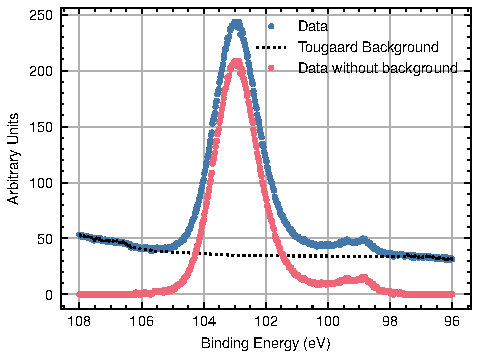
\includegraphics[width=\columnwidth]{Figuras/data_init.pdf}
    \caption{Dados com e sem Background removido}
    \label{fig:bgrm}
  \end{figure}

\subsection{Desconvolução de picos}

Observando-se a Fig. \ref{fig:bgrm} rapidamente se identifica 1 pico bem definido\footnote{São, na realidade, vários picos convoluídos}. No entanto também se observa a presença de uma estrutura de forma irregular entre os 98 e os $100\ \si{\electronvolt}$. É necessário compreender, distinguir e quantificar as contribuições que os diferentes estados de oxidação do Si têm nestas estruturas. Considerou-se, inicialmente a existência de Si em 5 estados diferentes: Si, Si$^{+1}$, Si$^{+2}$, Si$^{+3}$, Si$^{+4}$\footnote{Corresponde a SiO$_2$}. Os valores de \textit{binding energy} para os diferentes estados de oxidação foram inicialmente adaptados de \cite{Himpsel}, mas através de rotinas de \textit{fitting}, encontraram-se os valores ótimos para este caso. Tendo em conta que as orbitais em estudo são do tipo p (l=1) e que os eletrões possuem momento angular intrínseco (s=1/2), irão  existir \textbf{sempre} 2 tipos de acoplamento de momento angular possíveis $\qty(1\pm 1/2)$: 1/2 e 3/2. É possível também saber a razão entre a área dos picos para este acoplamento, devido ao número de estados de ocupação para cada um:


\begin{itemize}
  \item p 1/2$\longrightarrow 2\cdot 1/2 +1 = 2$ eletrões
  \item p 3/2$\longrightarrow 2\cdot 3/2 +1 = 4$ eletrões
\end{itemize}


Logo, será de esperar que a intensidade dos picos referentes a 2p 3/2 seja o dobro dos referentes a 2p 1/2. Também é conhecido, para o Si que, por norma existe uma diferença de $0.6\ \si{\electronvolt}$ entre os acoplamentos. Estes 2 factos referidos anteriormente foram usados como \textit{constraints} aquando a realização dos \textit{fits}.

\begin{figure}[t!]
  \centering
  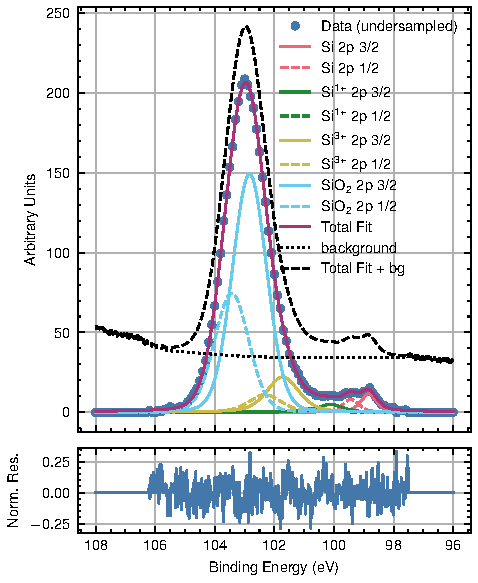
\includegraphics[width=\columnwidth]{Figuras/fits.pdf}
  \caption{Componentes e Fit total}
  \label{fig:tot}
\end{figure}


Observou-se que, para além de quase todo o Si na interface se encontrar completamente oxidado (Si$^{+4}$), ainda se encontra a presença de Si, Si$^{+1}$ e Si$^{+3}$, notando-se a ausência de Si$^{+2}$. Tendo em conta que as linhas possuem diferentes proporções de componentes Gaussianas e Lorentzianas, definiu-se que, a componente Gaussiana aumenta com a energia e fixou-se que os acoplamentos possuiam o mesmo tipo de linha e a mesma FWHM.

\begin{table}[h!]
  \centering
  \caption{Parâmetros do fit para as orbitais 2p 3/2 e comparação com valores de referência\cite{Nist}. É possível calcular-se os parâmetros das orbitais 2p 1/2 somando $0.6\ \si{\electronvolt}$ às centroides e dividindo as intensidades por 2. Os restantes parâmetros são os mesmos.}
  \begin{tabular}{lccccc}
    \hline\hline\noalign{\smallskip}
    \!\!State & \!\!\!\!Centroid &Cent. Diff& \!\!\!\!FWHM& \!\!\!\!Intensity\!\!\!\!&Line\\
    & \!\!\!\!$\qty(\si{\electronvolt})$&$\qty(\si{\electronvolt})$& \!\!\!\!$\qty(\si{\electronvolt})$& \!\!\!\!(Arb. u.)&Type\\
    \hline\noalign{\smallskip}
    \!\!Si &  -- && (2) & [16,64]&a\\
    \!\!Si$^{1+}$& [5,11]&& 3 & [10,40]&b\\
    \!\!Si$^{3+}$& [17,23]&& 3& [4,16]&c\\
    \!\!SiO$_2$ & [9,12] && 1 & [10,40]&d\\
    \hline
    \end{tabular}
    \label{table:params}
\end{table}


Os resultados obtidos (Tab. \ref{table:params} e Fig. \ref{fig:tot}) fazem sentido visto que, a remoção de eletrões no processo de oxidação leva a uma menor energia de repulsão entre os restantes, levando a um aumento da \textit{binding energy} para estados mais oxidados. Também se observa que a FWHM, tal como a componente Gaussiana, aumentam com o estado de oxidação. Também é de referir que os valores divergem ligeiramente de \cite{Himpsel} devido a diferentes contribuições de Estado Sólido.



\section{Quantificação}

Procedeu-se ao cálculo da estequiometria da interface com base numa simples aproximação mencionada em \cite{Himpsel}. Serão calculados os pesos de cada uma das intensidades sendo necessário primeiro proceder à sua normalização com base nas secções eficazes de ionização. Resumidamente:

\begin{gather}
  x_i= \qty(\frac{I_i}{\sigma_i})\cdot\qty(\sum_i^n \frac{I_i}{\sigma_i})^{-1} 
\end{gather}

Os valores de $\sigma_i$ para uma energia de feixe de $130\ \si{\electronvolt}$ foram consultados na \textit{TABLE II} de \cite{Himpsel}




%\begin{acknowledgement}

%\end{acknowledgement}



\bibliographystyle{unsrt}
\small
\bibliography{bibliografia}
 
\end{document}
